\documentclass[10pt,a4paper]{article}
\usepackage[utf8]{inputenc}
\usepackage[italian]{babel}
\usepackage{amsmath}
\usepackage{amsfonts}
\usepackage{amssymb}
\usepackage{siunitx}
\usepackage{graphicx}
\usepackage[left=2cm,right=2cm,top=2cm,bottom=2cm]{geometry}
\newcommand{\rem}[1]{[\emph{#1}]}
\graphicspath{ {../Figs-Tabs/} } % graphics search directories

\author{Gruppo BF \\ Andrea Luzio, Gianfranco Cordella, Valerio Lomanto}
\title{Esercitazione N.1: Misure di tensione, corrente, tempi, frequenza.}
\begin{document}

\maketitle

\section{Scopo e strumentazione}

L'esercitazione ha lo scopo di verificare la risposta in frequenza dei filtri passivi. Si misurano le caratteristiche principali di tali circuiti come guadagno in tensione e frequenze di taglio.

\section{Filtro passa-basso}
\paragraph{2.a }
Abbiamo montato il circuito in Fig. 1 con i valori di resistenza e capacità misurati con il multimetro digitale: $R_1 = 816\pm 7 \Omega$ , $R_2 = 99.7\pm 0.9 k\Omega$ e $C_1 = 110\pm 5 nF$. L'errore è stato stimato usando le indicazioni del manuale del multimetro.La frequenza di taglio attesa è $f_\mathrm{t}= \frac{1}{2\pi R_1C_1}= 1.77 \pm 0.09 kHz $.
Utilizzando l'oscilloscopio si sono misurati i rapporti tra le ampiezze della tensione in entrata e ai capi del condensatore a due frequenze diverse.
L'attenuazione intorno ai $2 kHz$ misurata è di $-3.4 dB$ contro un valore atteso di $-3.6 dB$. A $20 kHz$ si ha un valore atteso di $-21 dB$ contro una misura di $-20 dB$. 

\paragraph{2.b}
\'E stata misurata la frequenza di taglio (usando il frequenzimetro dell'oscilloscopio) come la frequenza compatibile ocn un'attenuazione di $-3dB$; essa risulta essere $f_t =1.88 \pm 0.05 kHz$. L'errore è stato stimato vedendo per quale variazione di frequenza si apprezza una variazione di ampiezza sull'oscilloscopio.
Si è inoltre misurata la suddetta frequenza di taglio con un fit a due rette(fit affine delle code $f<100 Hz$ e $f>14 kHz$  ) e con un fit della funzione di attenuazione (guadagno in $dB$). 
Si possono vedere i fit in \ref{f:fit1}. 
\begin{figure}
\centering
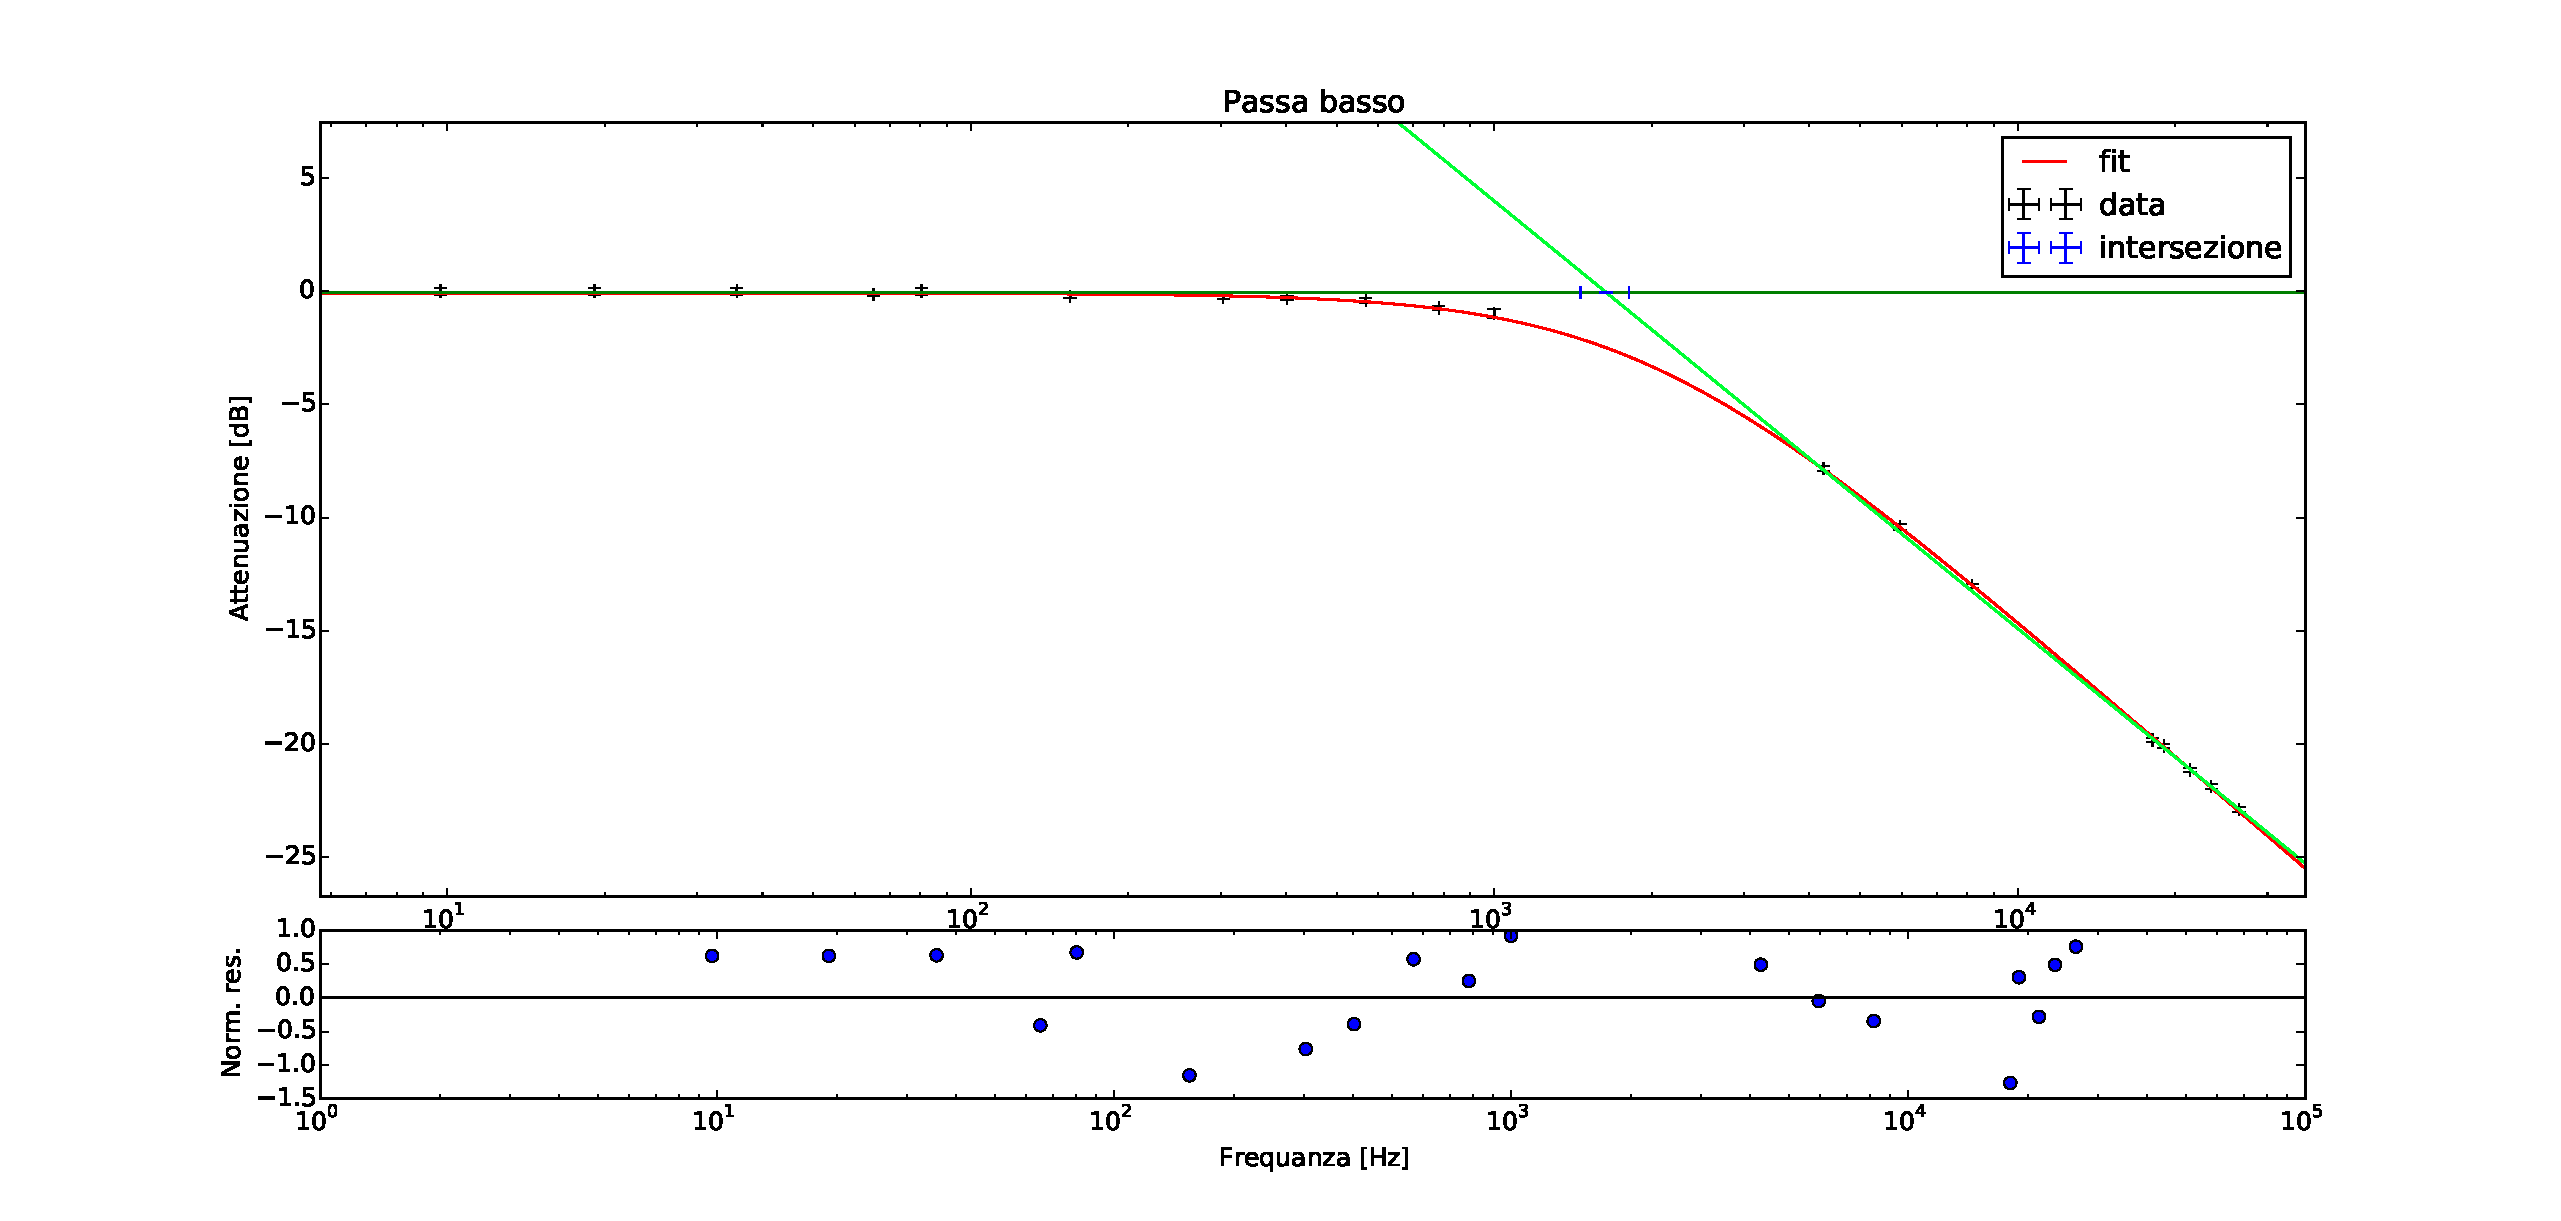
\includegraphics[scale=0.4]{plt_passa_basso.pdf}
\caption{Grafico di Bode e fit trasfermineto del passa-basso.\label{f:fit1}}
\end{figure}

I parametri trovati sono rispettivamente:\\
$f_t=1.64\pm 0.17 kHz$ e $f_t=1.90 \pm 0.01 kHz$. Nel fit dell'attenuazione si è ottenuto un $\chi^2=8 (/17 dof)$.
Si può notare che in alta frequenza la retta fittata ha una pendenza di $-18.9\pm 0.8 dB/decade$. Questo ci può suggerire che un possibile problema sia una sottostima della frequenza alla quale si può approssimare la funzione di trasferimento con la sua retta asintotica.

Il risultato trovato non è in perfetto accordo con il valore calcolato sulla base delle caratteristiche dei componenti scelti. Non ci sentiamo comunque di garantire una completa non compatibilità.


\paragraph{3 risposta al gradino }
Si è generata un'onda quadra e si è misurato il tempo di salita ,della tensione ai capi dell'oscilloscopio, usando i cursori dell'oscilloscopio. Il tempo di salita misurato è : $t_salita = 192 \pm 4 \mu s$.
Da cui si ricava $f_t = 1.82 \pm 0.04 kHz $. La misura è compatibile con il valore atteso di $1.77 \pm 0.09 kHz $.

\paragraph{4  }
L'impedenza di ingresso di un filtro passa-basso è : $Z_in = R_1 + \frac{f_t}{jf} $. A basse frequenze $Z_in$ diverge a infinito mentre ad alte frequenze il circuito è puramente resistivo.Per $f=f_t$ risulta invece $Z_in = R_1(1-j)$. 
La resistenza di carico in generale altera il funzionamento del circuito iniziale. Tuttavia se tale resistenza è molto maggiore della serie tra $R_1 e C_1$ allora la tensione all'uscita del condensatore viene completamente trasferita al carico stesso. Questa situazione rispecchia quella ideale in cui l'inserimento di un componente non altera il funzionamento del circuito iniziale. Perciò se abbasso la resistenza del carico a $10 k\Omega$, la differenza percentuale  $\frac{V_{out}(R_L)-V_{out}}{V_{out}} = \frac{R_1/R_L}{(V_{out})^4}$ risulta del $32 \%$ alla frequenza di taglio del circuito iniziale contro un valore del $3 \%$ per $R_L=100 k\Omega$.

\begin{figure}
\centering
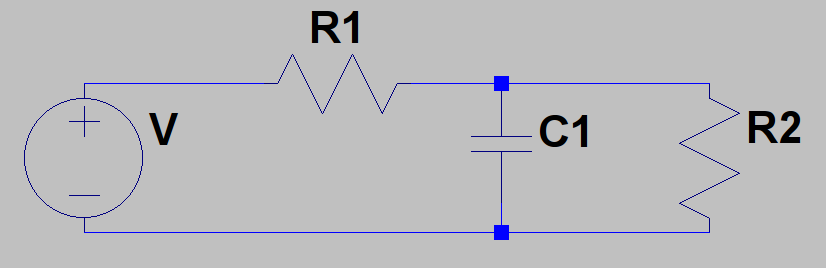
\includegraphics[scale=0.4]{passa_basso.png}
\caption{Filtro passa-basso.\label{f:par2}}
\end{figure}








\paragraph{2.c Partitore con resistenze pi\`u grandi}
Montando di nuovo il partitore con le resistenze $R_1 = 1.518\pm 0.01 M\Omega$ e $R_2 = 1.03\pm 0.01 M\Omega$, usando il voltmetro analogico per misurare $V_{OUT}$($20 kohm/volt$) si osservano i nuovi dati in tabella 2
\begin{table}[h]
\centering
\begin{tabular}{|c|c|c|c|}
\hline 
VIN[V]& $\sigma$ VIN[mV] & VOUT[V]	 & $\sigma$ VOUT[mV] \\
\hline 
10.02 & 60 & 0.24 & 2 \\
8.90 & 55 & 0.20 & 2 \\
7.90 & 50 & 0.18 & 1 \\
6.80 & 44 & 0.16 & 1 \\
6.06 & 40 & 0.14 & 1 \\
4.52 & 30 & 0.1 & 0.6 \\
3.52 & 30 & 0.08 & 0.5 \\
\hline 
\end{tabular} 
\caption{Partitore di tensione. Tutte le tensioni in V.\label{t:par2}}
\end{table}
\begin{figure}
\centering
%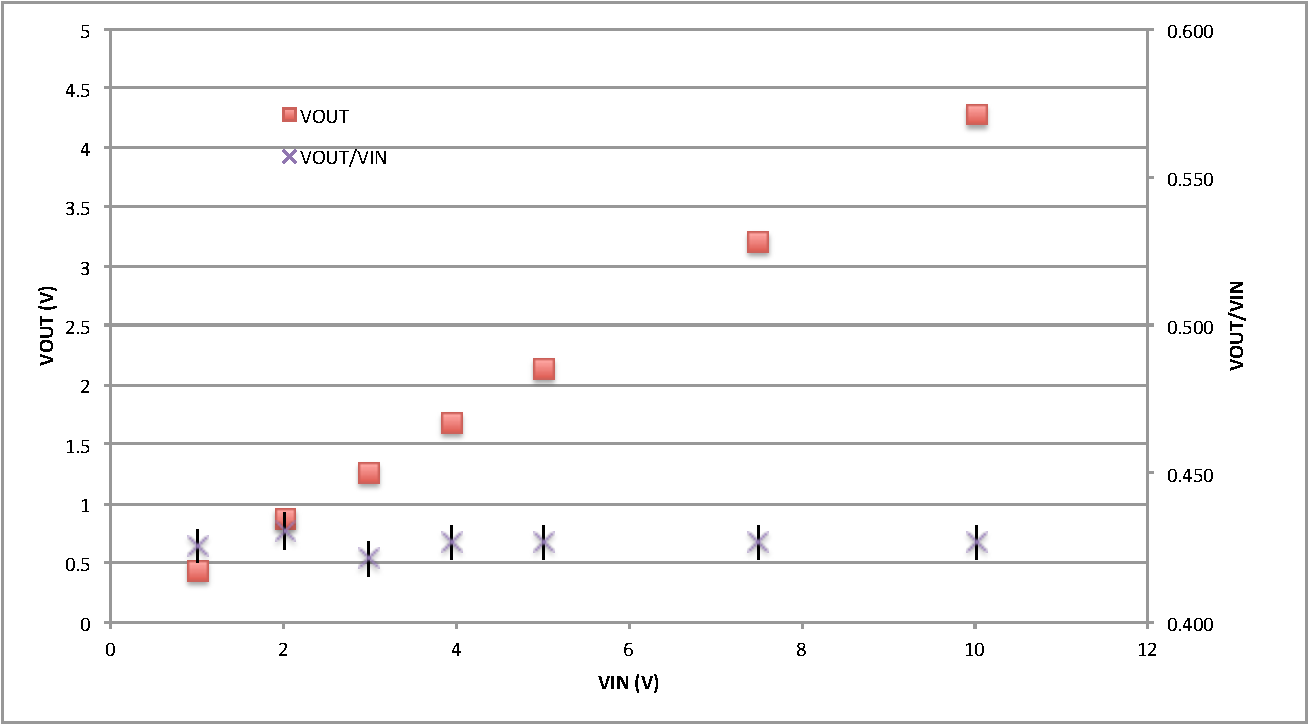
\includegraphics[scale=0.4]{part2.pdf}
\caption{Partitore di tensione con resistenze da circa 1M.\label{f:par2}}
\end{figure}

Si osserva come valore del rapporto misurato con le resistenze da $1 M\Omega$, $0.0229 \pm 1e-04$ si discosti da quanto atteso   $V_\mathrm{OUT}/V_\mathrm{IN} = \frac{1}{1+R_1/R_2}= 0.40 $\footnote{\'E stato omesso l'errore poich\'e il calcolo \'e stato fatto senza considerare la resistenza di ingresso del voltmetro, li risultato \'e tuttavia chiaramente incompatibile con l'ipotesi che il voltmetro sia uno strumento ideale}. La ragione della discrepanza \`e da ricercarsi nella impedenza di ingresso del tester.


\paragraph{2.d Resistenza di ingresso del tester}

 Usando il modello mostrato nella scheda si ottiene
\[ \frac{R_1}{R_T} =  \frac{V_{IN}}{V_{OUT}} - (1 +  \frac{R_1}{R_2} )
\]
Il valore misurato \'e dunque $R_T=38.3 \pm 0.6 kohm$, vicino ai valori di riferimento del tester analogico( $40 kohm$ con il fondoscala $2 V$, dato fornito dal manuale senza incertezza).

\subsection{Partitore di corrente: 2.e}

Si monta il circuito indicato con i valori di resistenza misurati con il multimetro digitale: 
$R_3= 98.3\pm 1 k\Omega$, $R_1 = 560\pm 5 \Omega$, $R_2 = 220\pm 3 \Omega$.
Si \'e variata la tensione fornita dal generatore nel range $20-10 V$ per ottenere pi\'u misure e poter procedere con un fit.
Il valore di tensione $V_{in}$ è stato misurato con il multimetro digitale, mentre la corrente con l'analogico, fornendo esso misure pi\'u precise per basse correnti in continua.\\
 

\begin{center}
\begin{tabular}{|c|c|c|c|c|c|}
\hline 
$V_{in} (V)$ & $\sigma V_{in} (V)$& I1 ($\mu A$)& $\sigma$(I1) ($\mu A$) & I2	($\mu A$) & $\sigma$(I2) ($\mu A$)  \\
\hline 
19.2 & 0.1 & 26.0 & 0.3 & 10.0 & 0.1 \\
17.2 & 0.1 & 23.5 & 0.2 & 9.0 & 0.1 \\
14.9 & 0.1 & 20.5 & 0.2 & 8.0 & 0.1 \\
12.65 & 0.07 & 17.0 & 0.2 & 7.00 & 0.07 \\
10.87 & 0.06 & 15.00 & 0.15 & 6.00 & 0.06 \\
\hline 
\end{tabular} 
\end{center}

Ci si accorge subito che $I_1=I_{tot,1}\frac{R_2}{R_{int}+R_1+R_2}$ (dove $R_{int}$\footnote{dove $I_{tot, 1}$ \'e la corrente che passa da $R_3$ quando l'amperometro \'e nel ramo di $R_1$, similmente $I_{tot, 2}$ } \'e la resistenza interna dell'amperometro, c.a. $2 kohm$ con il fondoscala usato). Anche $I_2=I_{tot,2}\frac{R_1}{R_{int}+R_1+R_2}$. \'E lecito approssimare $I_{tot, 1}=I_{tot, 2}=I_{tot}$ poich\'e la resistenza $R_3$ domina sul parallelo in entrambi i casi.
Dalle equazioni scritte sopra si nota che $\frac{I_1}{I_2}=\frac{R_2}{R_1}$ ma non \'e vero che $I_1+I_2=I_{tot}$. Infatti sperimentalmente(facendo un fit lineare ad un parametro, si veda figura 1 e 2, di $I_1=K I_2$:
$\frac{I_1}{I_2}=1.99 \pm 0.05$
compatibile con il valore atteso di $\frac{R_2}{R_1}=2.00 \pm 0.02$.
\begin{figure}
\centering
%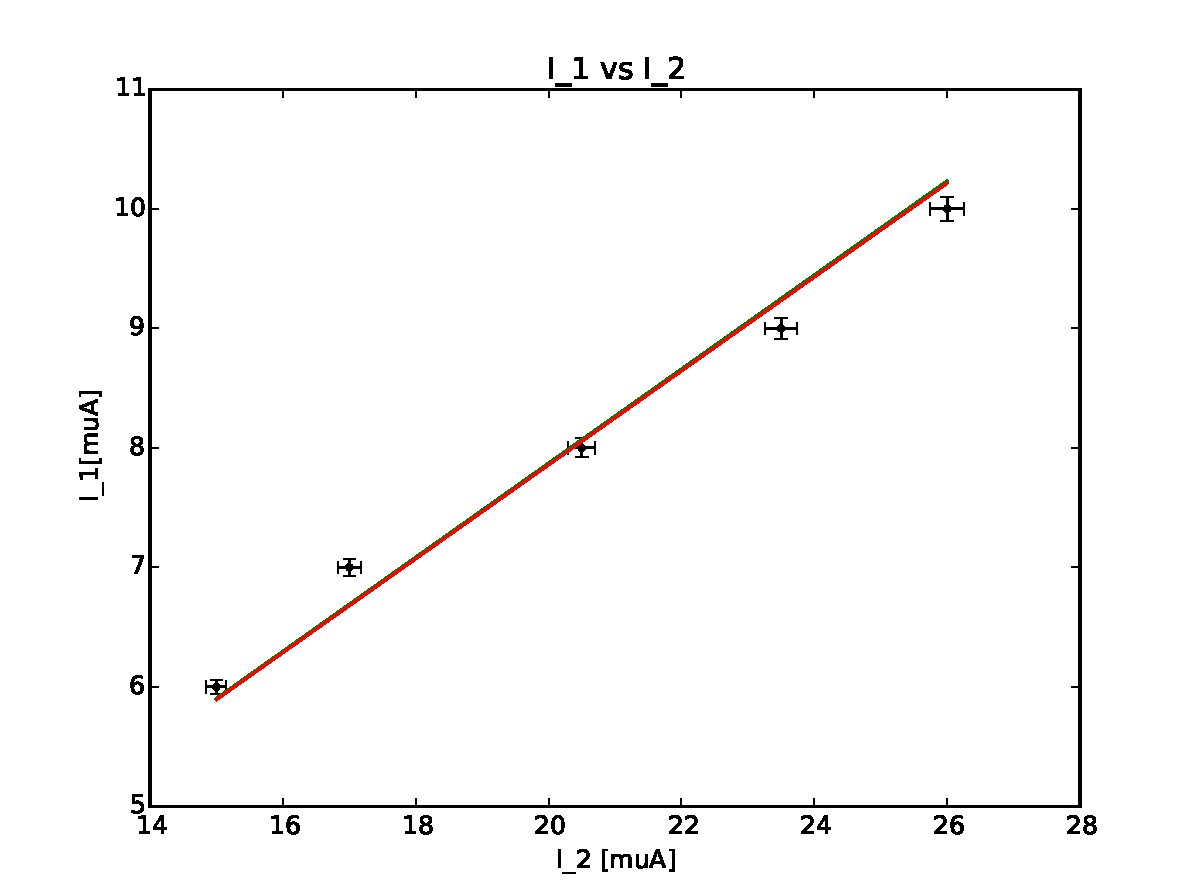
\includegraphics{/home/gianfranco/Scaricati/immagini/fig2e.pdf}
\caption{Fit e dati di $I_1 vs I_2$}
\end{figure}
\begin{figure}
\centering
%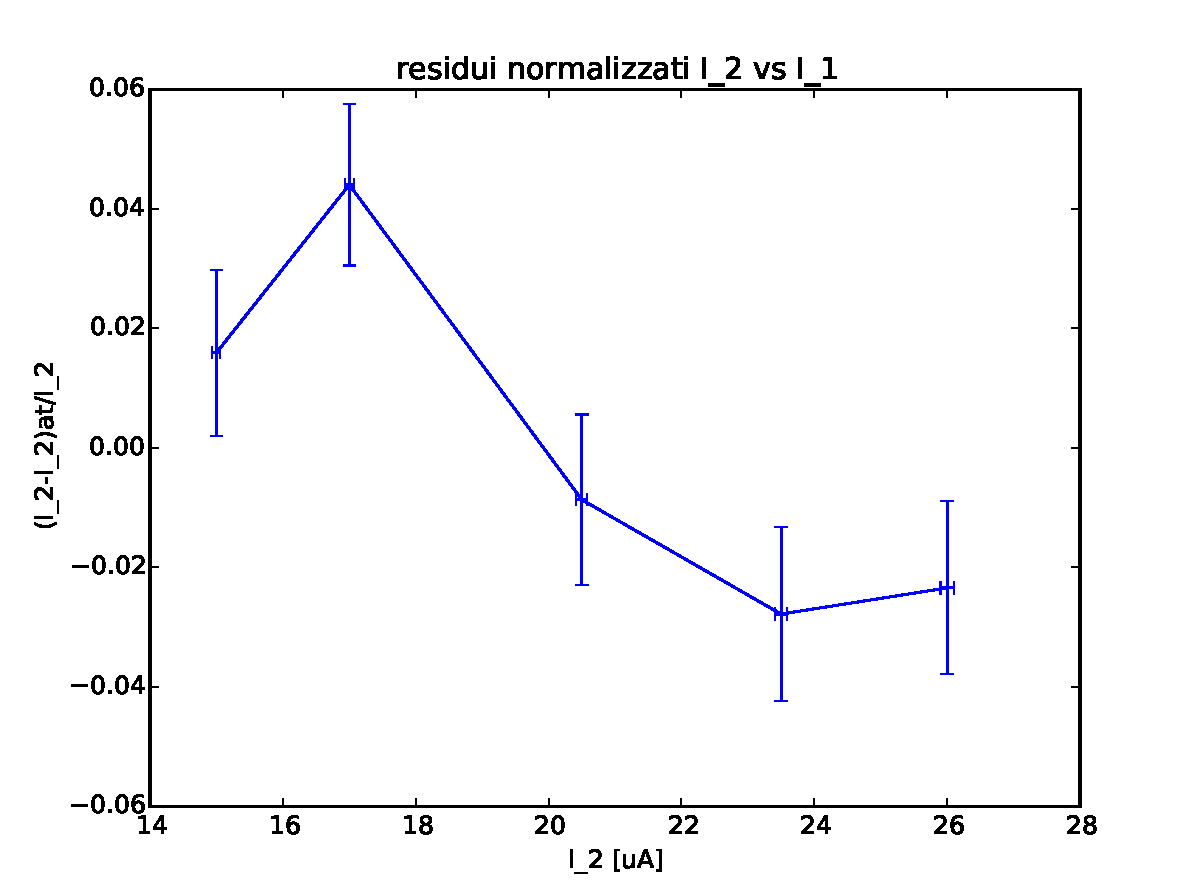
\includegraphics{/home/gianfranco/Scaricati/immagini/fig2eres.pdf}
\caption{Residui di $I_1 vs I_2$}
\end{figure}
Chiaramente $I_1+I_2\neq I_{tot}$ ad esempio, per la prima misura, $\frac{I_1+I_2}{I_{tot}}=0.18$
Si pu\'o calcolare, sfruttando questa discrepanza la resistenza interna dell'amperometro. Sempre nell'approssimazione che $I_{tot}$ non cambi spostando l'amperometro (questo \'e vero con un incertezza maggiore del 0.5 \%) la resistenza interna dell'amperometro \'e $R_A = (R1+R2)\left(\frac{I_{TOT}}{I1+I2} - 1 \right)$. Dunque $R_A=3.4 kohm$ al $1.2 \%$.



\section{Uso dell'oscilloscopio}

\paragraph{Misure di tensione}
Usando i seguenti resistori per fare un partitore di tensione $ 
R_2=9.91\pm 0.08 kohm
R_1=9.90\pm 0.08 kohm$
si ottengono le seguenti misure:
\begin{table}[h]
\centering
\begin{tabular}{|c|c|c|c|}
\hline 
VIN[V]& $\sigma$ VIN[mV] &VOUT[V]	 & $\sigma$ VOUT[mV] \\
\hline 
11.6 & 0.7 & 5.92 & 0.3 \\
9.8 & 0.6 & 4.8 & 0.3 \\
8.1 & 0.4 & 4.0 & 0.2 \\
5.4 & 0.3 & 2.7 & 0.14 \\
4.2 & 0.2 & 2.1 & 0.1 \\
2.64 & 0.14 & 1.33 & 0.07 \\
1.76 & 0.10 & 0.88 & 0.05 \\
\hline 
\end{tabular} 
\caption{Partitore di tensione usato con l'oscilloscopio.\label{t:par1}}
\end{table}
Il rapporto di partizione misurato \'e $1.99\pm 0.04 $ contro un valore atteso di $2.00 \pm 0.02$.


\paragraph{Impedenza di ingresso dell'oscilloscopio}
L'impedenza di ingresso dell'oscilloscopio \'e stata misurata con un partitore di tensione con $R_1=0.985\pm 0.01 Mohm R_2=0.560\pm 0.005 Mohm$. Il CH2 dell'oscilloscopio (quello del quale abbiamo misurato l'impedenza di ingresso) era ai capi di $R_1$. Con CH1 si misurava invece la tensione di ingresso al partitore.
La resistenza risultante \'e $1.0 \pm 0.1 Mohm$.  

\section{Misure di frequenza e tempo}
Sono stati misurate le seguenti frequenze:
\begin{table}[h]
\centering
\begin{tabular}{|c|c|c|c|}
\hline 
$f_{oscilloscopio}[kHz] $& $f[kHz]$ &$\sigma f [kHz]$ \\
\hline 
1.559 & 1.53 & 0.01 \\
15.09 & 15.3 & 0.1 \\
150.4 & 148 & 1 \\
1506.0 & 1490 & 10 \\

\hline 
\end{tabular} 
\caption{Frequenze misurate con il frequenzimetro e con i cursori. Non \'e noto l'errore del frequenzimetro.\label{t:par1}}
\end{table}

\section{Trigger dell'oscilloscopio}
Generando un onda quadra con frequenza $1 MHz$ si sono ottenuti i seguenti tempi di salita e discesa:


\begin{table}[h]
\centering
\begin{tabular}{|c|c|c|}
\hline 
tipo misura& manuale[ns] & automatico[ns] \\
\hline 
salita & $68 \pm 1$ & $66 \pm 2$ \\
discesa & $62 \pm 1$ & $62 \pm 2$\\

\hline 
\end{tabular} 
\caption{La misura automatica \'e presa con l'opportuna funzione dell'oscilloscopio, la manuale con i cursori. \label{t:par1}}
\end{table}
\section{Conclusioni e commenti finali}
Di questa esperienza non abbiamo capito molto, sfortunatamente non abbiamo fatto saltare alcun fusibile. 

\end{document}
